\lecture{10}{7 Oct. 15:30}{}
\section{Generating function operation}
\begin{itemize}
    \item Substituting \(x^k\) for \(x\), then 
    \[
        (a_0, a_1, \dots ) \to \left(a_0, \underbrace{0, 0, \dots , 0}_{k}, \dots, \begin{dcases}
            0 , &\text{ if } k \nmid n ;\\
            a_{\frac{n}{k}}, &\text{ if } k \mid n.
        \end{dcases}\right)
    \]
    since for \(A(x) = \sum_{i=0}^{\infty} a_i x^i \), we have 
    \[
        A \left( x^k \right) = \sum_{i=0}^{\infty} a_i \left( x^k \right)^i = \sum_{i=0}^{\infty} a_i x^{ki}.   
    \] 
    \item Differentiation: 
    \[
        (a_0, a_1, \dots) \to (a_1, 2 a_2, 3 a_3, \dots ).
    \]
    \item Integration: 
    \[
        (a_0, a_1, \dots ) \to \left( 0, \frac{a_1}{1}, \frac{a_2}{2}, \dots  \right) 
    \] since
    \[
        \int _0 ^x A(t) \, \mathrm{d} t = \sum_{n=0}^{\infty} \int _0 ^ x a_n t^n \, \mathrm{d} t = \sum_{n=0}^{\infty} a_n \left[ \frac{t^{n+1}}{n + 1} \right]_0 ^ x = \sum_{n=0}^{\infty} \frac{a_n}{n + 1} x^{n + 1}.      
    \]
\end{itemize}

\begin{eg}
    Find the generating functions for the sequences:
    \begin{itemize}
        \item [(i)] \(a_n = 2^{\left\lfloor \frac{n}{2} \right\rfloor}\)
        \item [(ii)] \(a_n = (n + 1)^2\). 
    \end{itemize}
\end{eg}
\begin{explanation}
    \vphantom{text}
    \begin{itemize}
        \item [(i)] Note that \((a_i)_{i=0}^{\infty} = (1, 1, 2, 2, 4, 4, 8, 8, 16, 16, \dots )\), and we can write it as 
        \[
            (1,0,2,0,4,0,8,0,16,0,\dots ) + (0, 1, 0, 2, 0, 4,0, 8, 0, 16,\dots ),
        \] where the first term is \(B(x) = (1, 2, 4, 8, 16, \dots )\) spread by \(2\), which is \(B \left( x^2 \right) \), and the second term is \(x B \left( x^2 \right) \). Note that \(B(x) = \frac{1}{1 - 2x}\).  
        \item [(ii)] If \(b_n = n\) corresponds to \(B(x)\), then 
        \[
            A(x) = \frac{\mathrm{d}B(x)}{\mathrm{d}x} 
        \] has \(a_n = (n + 1) b_{n+1} = (n+1)^2\). Also, if the sequence \(c_n = 1\) has generating function \(C(x) = \frac{1}{1-x}\), then 
        \[
            \frac{\mathrm{d}}{\mathrm{d}x} C(x) \sim (1,2,3, \dots ),
        \] so 
        \[
           B(x) = x \frac{\mathrm{d}}{\mathrm{d}x} C(x),
        \]
        and we have 
        \[
            A(x) = \left[ x \left( \frac{1}{1 - x} \right)^{\prime}   \right]^{\prime} = \frac{2}{(1-x)^3} - \frac{1}{(1-x)^2}. 
        \]  
    \end{itemize}
\end{explanation}

\section{Products of Generating Functions}
Suppose \(A(x) = \sum_{n=0}^{\infty} a_n x^n \) and \(B(x) = \sum_{n=0}^{\infty}  b_n x^n \),
\begin{question}
    What can we say about \(C(x) = A(x) B(x)\)?  
\end{question}
\begin{align*}
    A(x) B(x) &= \left( \sum_{n=0}^{\infty} a_n x^n  \right) \left( \sum_{n=0}^{\infty} b_n x^n  \right) \\
    &= \sum_{n, m \ge 0} a_n b_m x^{n + m} \\
    &= \sum_{r \ge 0} \left( \sum_{\substack{n, m \ge 0 \\ n + m = r}} a_n b_m  \right) x^r = \sum_{r \ge 0} \left( \sum_{m=0}^r a_n b_{r - n}  \right) x^r \\
    &= \sum_{n=0}^{\infty} \left( \sum_{k=0}^n a_k b_{n - k}  \right) x^n        
\end{align*} 
i.e. \(C(x)\) corresponds to the sequence \(c_n = \sum_{k=0}^n a_k b_{n - k} \), and we call it a convolution. 

\subsubsection{Combinatorial interpretation}
Suppose \((a_n)\) represents the number of ways of completing task \(1\) with a budget of \(\$ n\), and \((b_n)\) represents the number of ways of completing task \(2\) with a budget of \(\$ n\). Then the convolution \(c_n = \sum_{k=0}^n a_k b_{n-k} \) represents the number of ways of completing both task \(1\) and \(2\) with a combinatorial budget of \(\$ n\). 
\begin{eg}
    Designing a physics course for \(n\) days, which has theoretical part including one midterm exam and it is followed by a practical part, which includes two experiments. This is a convolution of the sequences 
    \[
        (a_n) = \# \text{ of ways of planning theory} \text{ and } (b_n) = \# \text{ of ways of planning practical}.
    \] Note that \(a_n = n\) and \(b_n = \binom{n}{2}\), so 
    \[
        A(x) = x \left( \frac{1}{1-x} \right)^{\prime} = \frac{x}{(1-x)^2} \quad B(x) = \frac{x^2}{(1-x)^3}
    \] since \(b_n = \binom{n}{2} = \frac{n(n-1)}{2}\). Hence, \(C(x) = \frac{x^3}{(1-x)^5}\) is the generating function for the sequence \((c_n)\) where \(c_n\) is the number of ways of designing an \(n\)-day course. Now since 
    \[
        C(x) = \frac{x^3}{(1-x)^5} = x^3 (1 - x)^{-5}
    \] and 
    \[
        (1-x)^{-5} = \sum_{n=0}^{\infty} \binom{-5}{n} (-x)^n, 
    \]  and 
    \[
        \binom{-5}{n} = \frac{(-5)(-5 - 1)(-5 - 2) \dots (-5 - (n-1))}{n!},
    \] so we have 
    \[
        \binom{-5}{n} (-x)^n = \frac{5(5+1)\dots (5 + (n-1))}{n!} x^n = \binom{n+4}{n} x^n,
    \] and we have to shift it by \(3\), so 
    \[
        c_n = \binom{n+1}{n-3} = \binom{n+1}{4}.
    \] 
\end{eg}       
\begin{remark}
    If we think of putting \(4\) bars in \(n+1\) space, then it can be easily thought that \(c_n = \binom{n+1}{4}\).   
    \begin{note}
        We can think of there are \(n + 1\) spaces, and the boundary between the theoretical part and the practical part is \(\mid\), and the midterm of theoretical part is \(a\), while the experiments of practical part are \(b_1, b_2\), and the other symbols are \(*\), which are some normal course days, then we can first choose \(4\) spaces out of \(n + 1\) spaces, and put on \(a, \mid , b_1, b_2\) in order, then use \(*\) to fill all the other spaces. Note that this method corresponds to a way of designing the courses, so \(c_n = \binom{n + 1}{4}\).            
    \end{note}
\end{remark}  
\section{Catalan Numbers}
\begin{eg}
    Bank balance goes up by \(\$ 1\) or down by \(\$ 1\), and bank balance should always be \(\ge 0\).    
\end{eg}
\begin{question}
    Start with \(\$ 0\). How many ways can we have \(\$ 0\) after \(2n\) days?   
\end{question}
\begin{answer}
    Define \(c_n = \) number of ways of having \(\$ 0\) after \(2n\) days. Consider the first timewe have \(\$ 0\). Suppose it happens on Day \(2k\), \(k \ge 1\), then \(c_{n-k}\) ways proceeding from Day \(2k\) to Day \(2n\), where \(c_0 = 1\). For the initial period: Since we know during Day 1 to Day \(2k - 1\), we've never been to \(\$0\), and in Day 1, we should have \(+1\), and in Day \(2k\), we must have \(-1\), so in between, we must have at least \(\$1\), so it is Dyck path from Day 1 to Day \(2k - 1\) with axis \(y = 1\). Hence, by the sum rule, 
    \[
        c_n = \sum_{k=1}^{n} c_{k-1} c_{n - k} \quad \forall n \ge 1 \text{ with } c_0 = 1.
    \]       
    
    \begin{figure}[H]
    \centering
    % First image
    \begin{minipage}[b]{0.45\textwidth} % width = 45% of line width
        \centering
        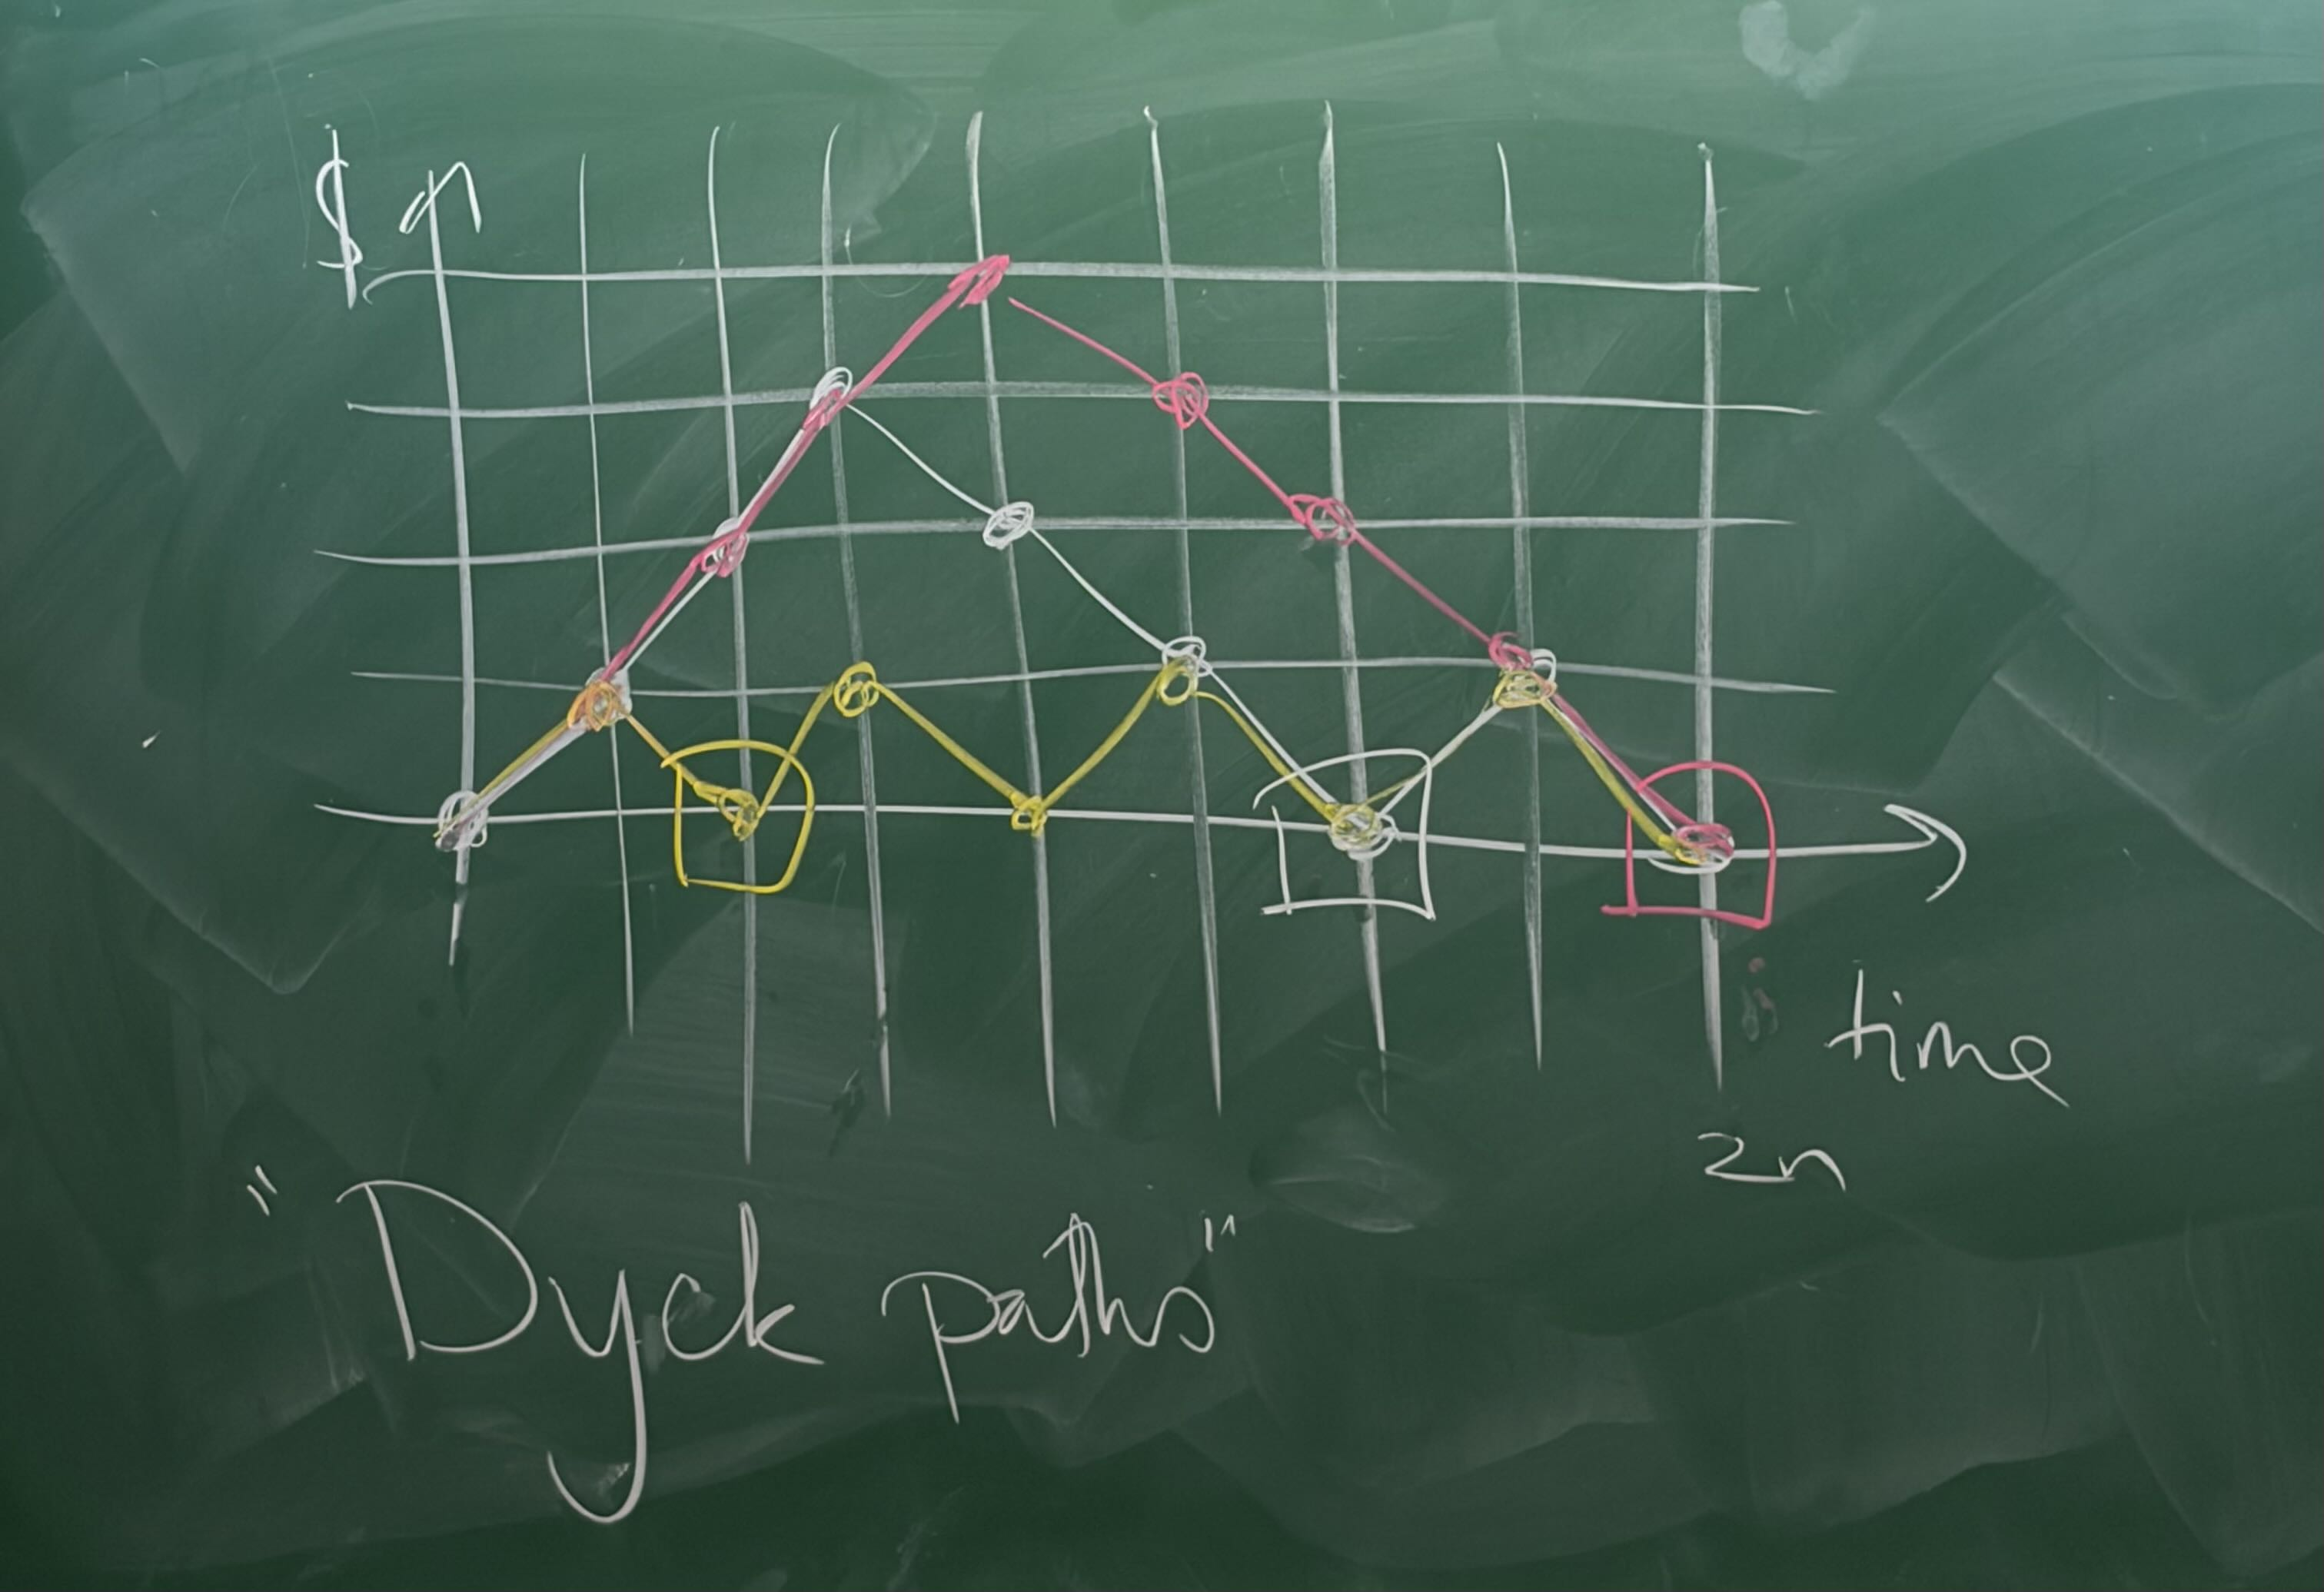
\includegraphics[width=\textwidth]{./Figures/IMG_0123.jpg}
        %\caption{First image}
        %\label{fig:first}
    \end{minipage}
    \hfill % adds horizontal space between the two minipages
    % Second image
    \begin{minipage}[b]{0.45\textwidth}
        \centering
        
\includegraphics[width=\textwidth]{./Figures/IMG_0124.jpg}
        %\caption{Second image}
        %\label{fig:second} 
    \end{minipage}
\end{figure}
\end{answer}

\begin{figure}[H]
    \centering
    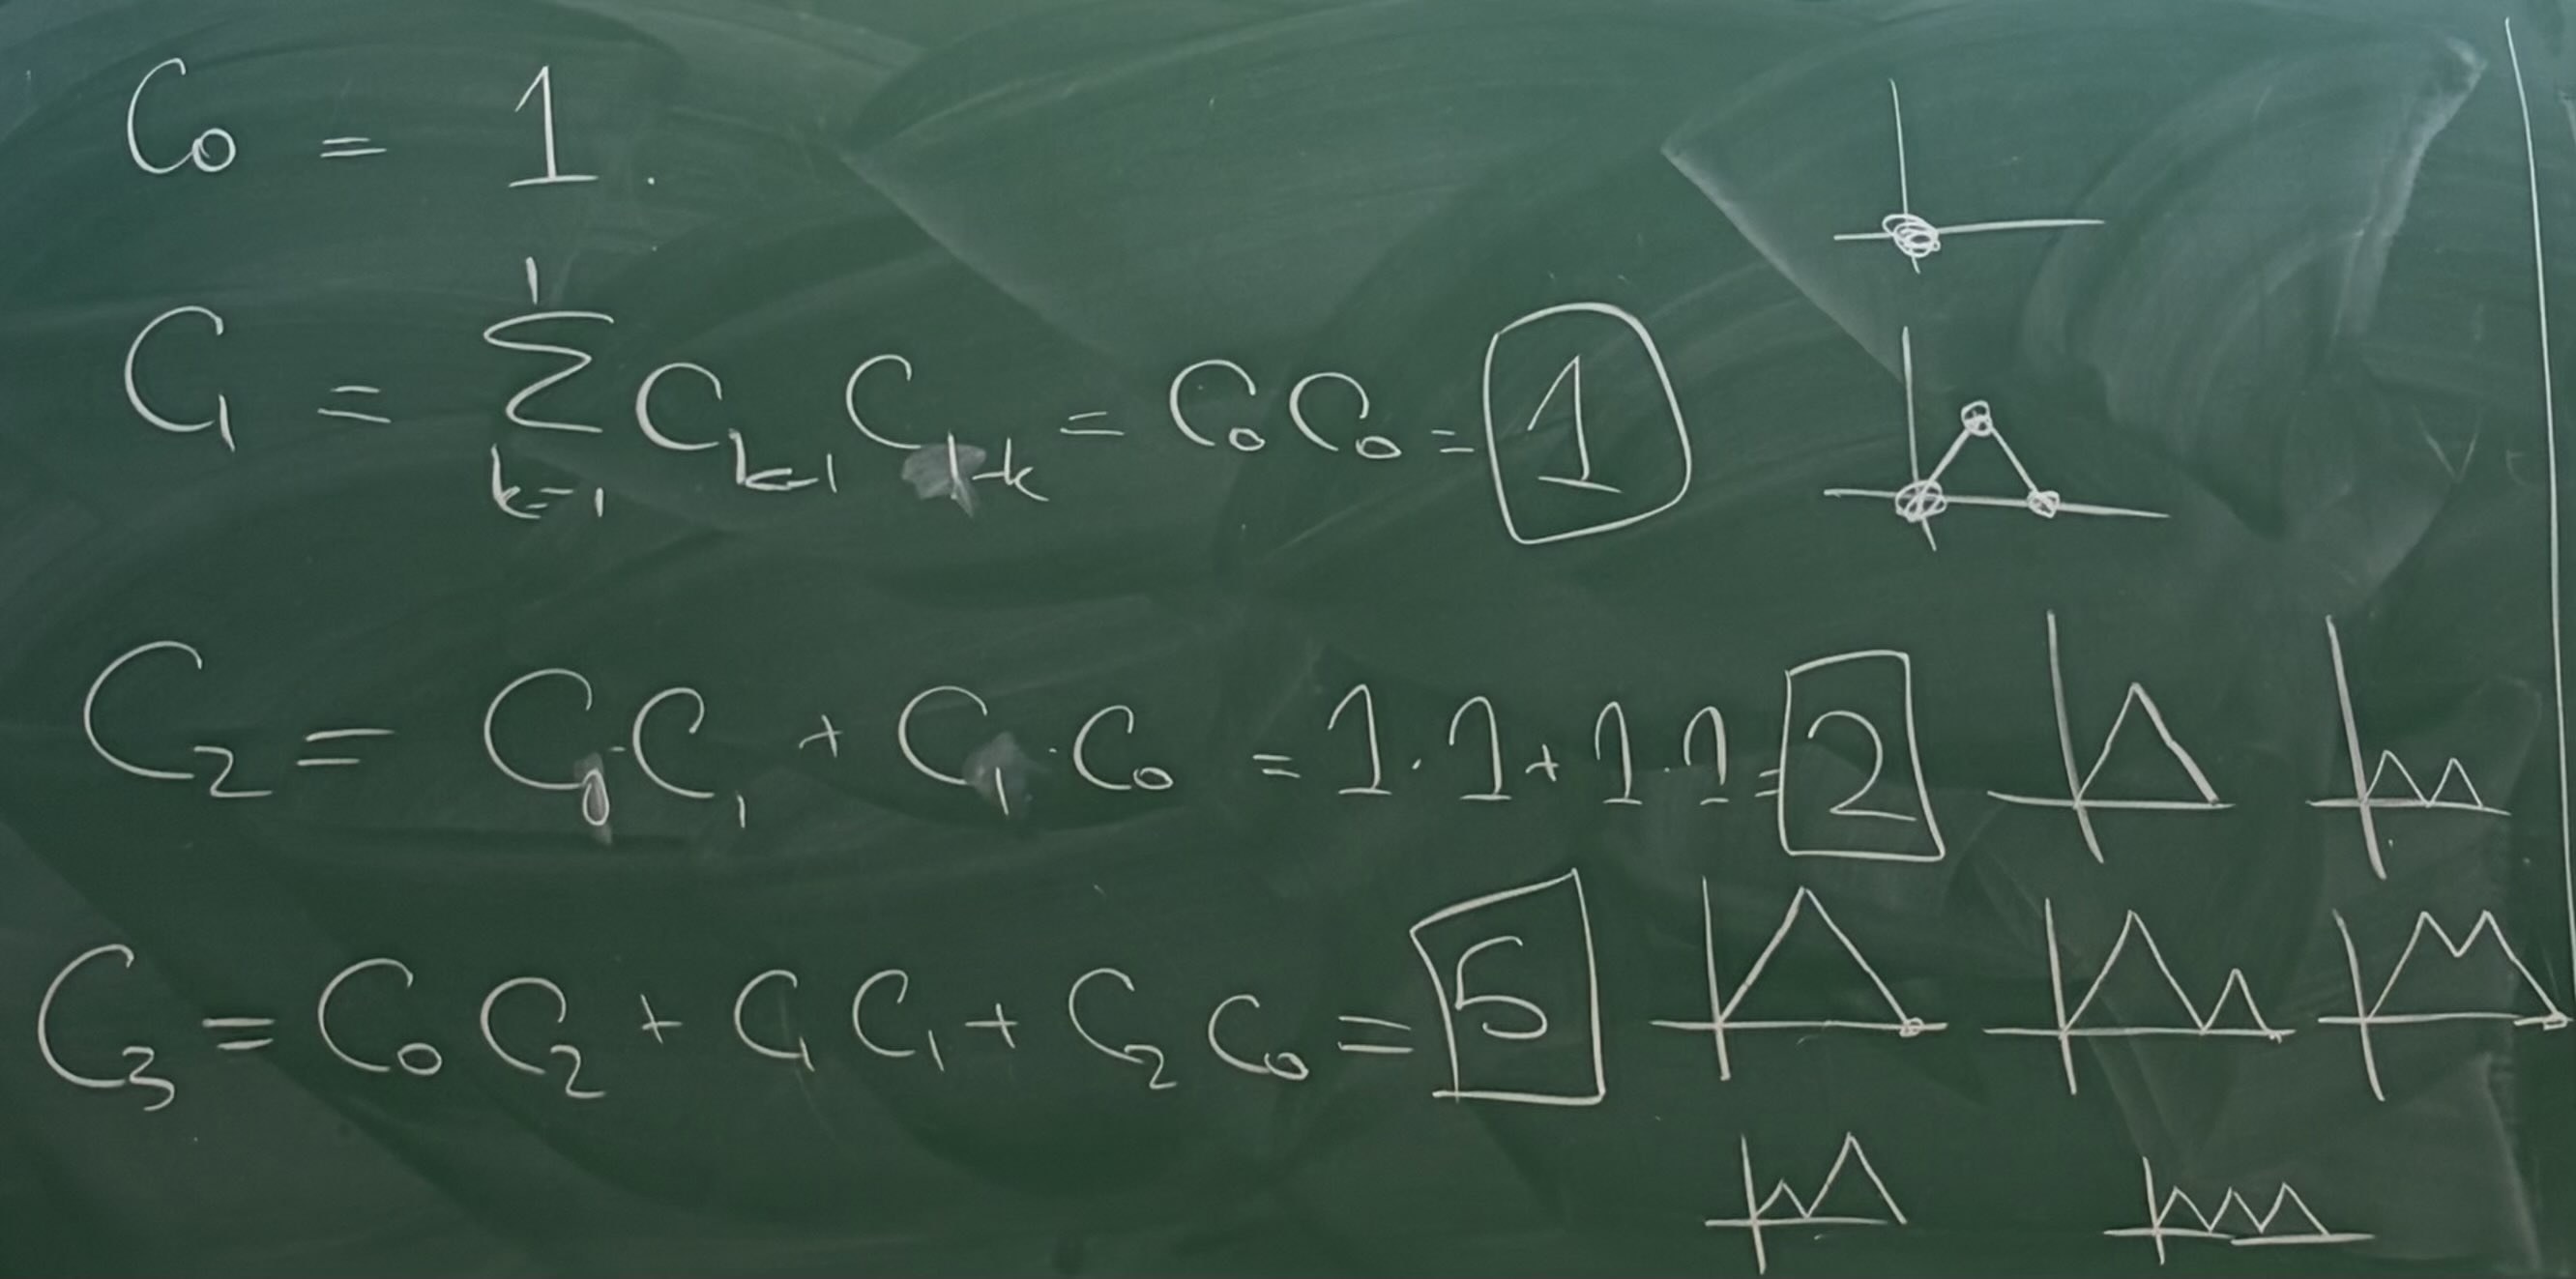
\includegraphics[width=0.8\textwidth]{./Figures/IMG_0125.jpg}
    \caption{Example of \(c_i\).}
\end{figure}